\section{Instance Segmentation}
\begin{frame}{}
    \LARGE Image Segmentation: \textbf{Instance Segmentation}
\end{frame}

\begin{frame}{Instance Segmentation}
    \begin{columns}
    \begin{column}{0.5\textwidth}
        \begin{itemize}
            \item<1-> Detect all objects in the image, and identify the pixels that belong to each object (Only things!)
            \item<2-> \textbf{Approach:} Perform object detection, then predict a segmentation mask for each object!
        \end{itemize}
    \end{column}
    \begin{column}{0.5\textwidth}
        \onslide<1->{
        \begin{figure}
        \centering
        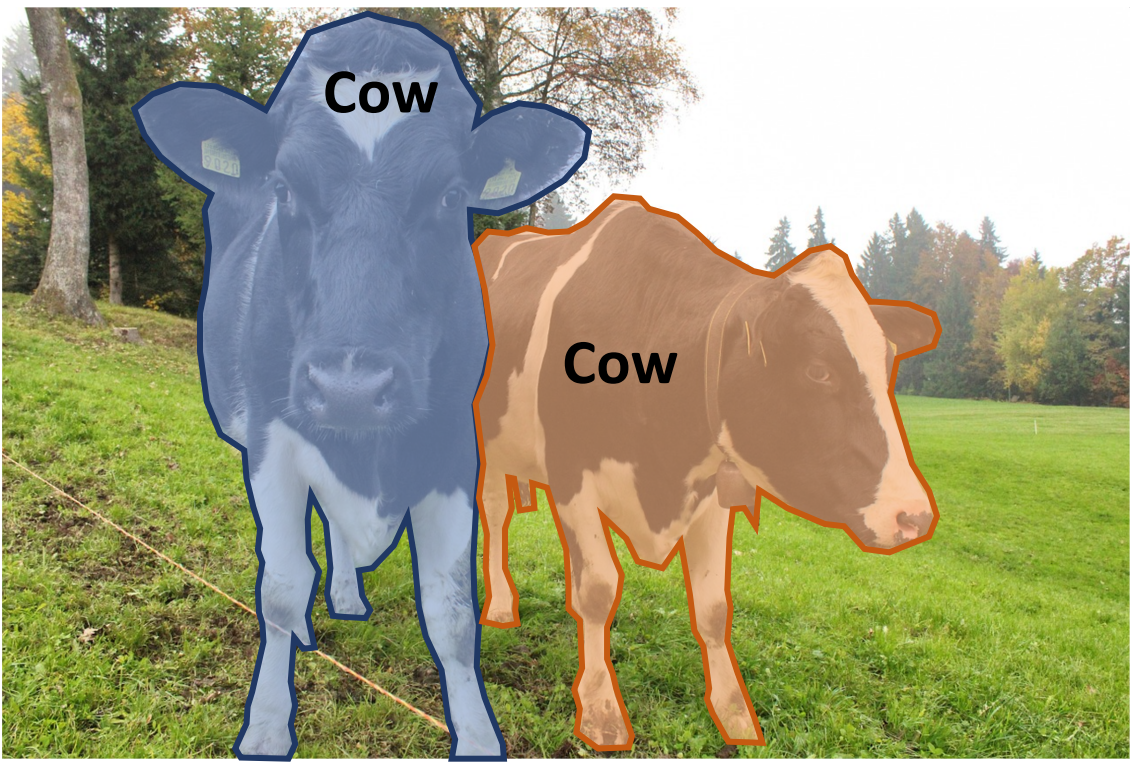
\includegraphics[width=1.0\textwidth,height=1.0\textheight,keepaspectratio]{images/segmentation/ins_4.png}
        \end{figure}
        }
    \end{column}
\end{columns}
\end{frame}

\subsection{Mask R-CNN}
\begin{frame}{}
    \LARGE Instance Segmentation: \textbf{Mask R-CNN}
\end{frame}

\begin{frame}[allowframebreaks]{Mask R-CNN}
    \textbf{Mask R-CNN Overview}
    \begin{itemize}
        \item \textbf{Developed on top of Faster R-CNN}
        \item Faster R-CNN outputs:
        \begin{itemize}
            \item Class label
            \item Bounding-box offset
        \end{itemize}
        \item Mask R-CNN adds a third branch:
        \begin{itemize}
            \item Predicts object mask for each candidate
        \end{itemize}
        \item Performs both \textbf{Semantic} and \textbf{Instance Segmentation}
    \end{itemize}

\framebreak

    \only<1>{
        \begin{figure}
        \centering
        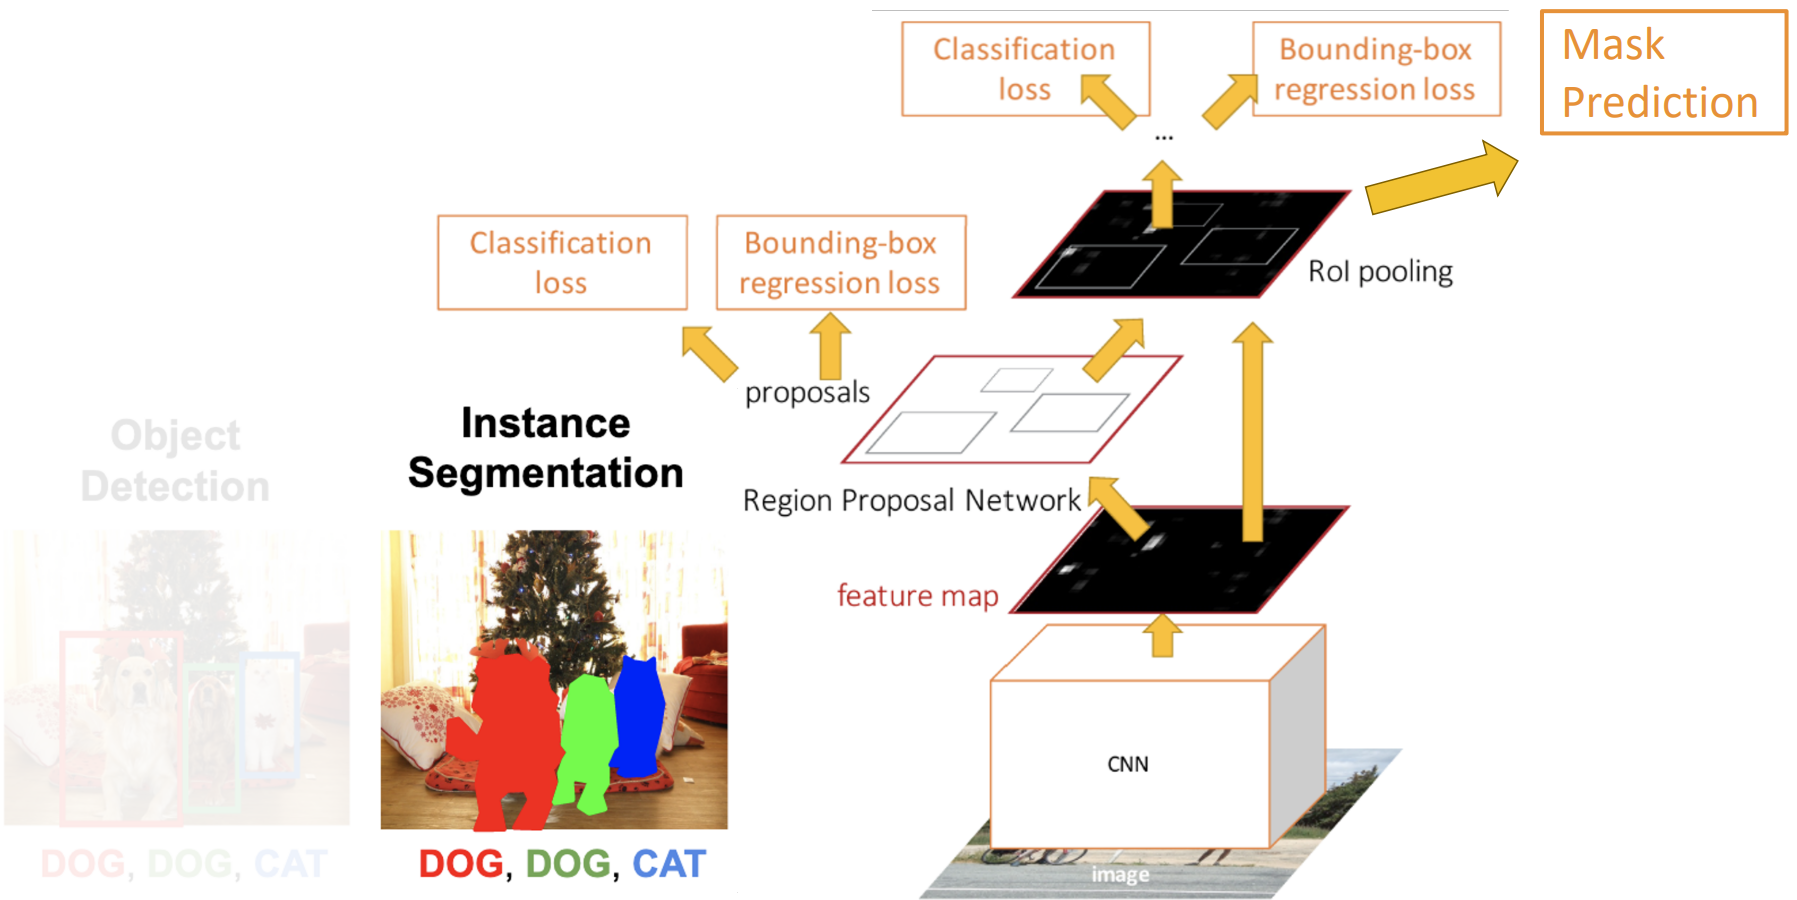
\includegraphics[width=1.0\textwidth,height=1.0\textheight,keepaspectratio]{images/object-detect/ins_6.png}
        \footnotetext{He et al, “Mask R-CNN”, ICCV 2017}
        \end{figure}
    }
    
    \only<2>{
        \begin{figure}
        \centering
        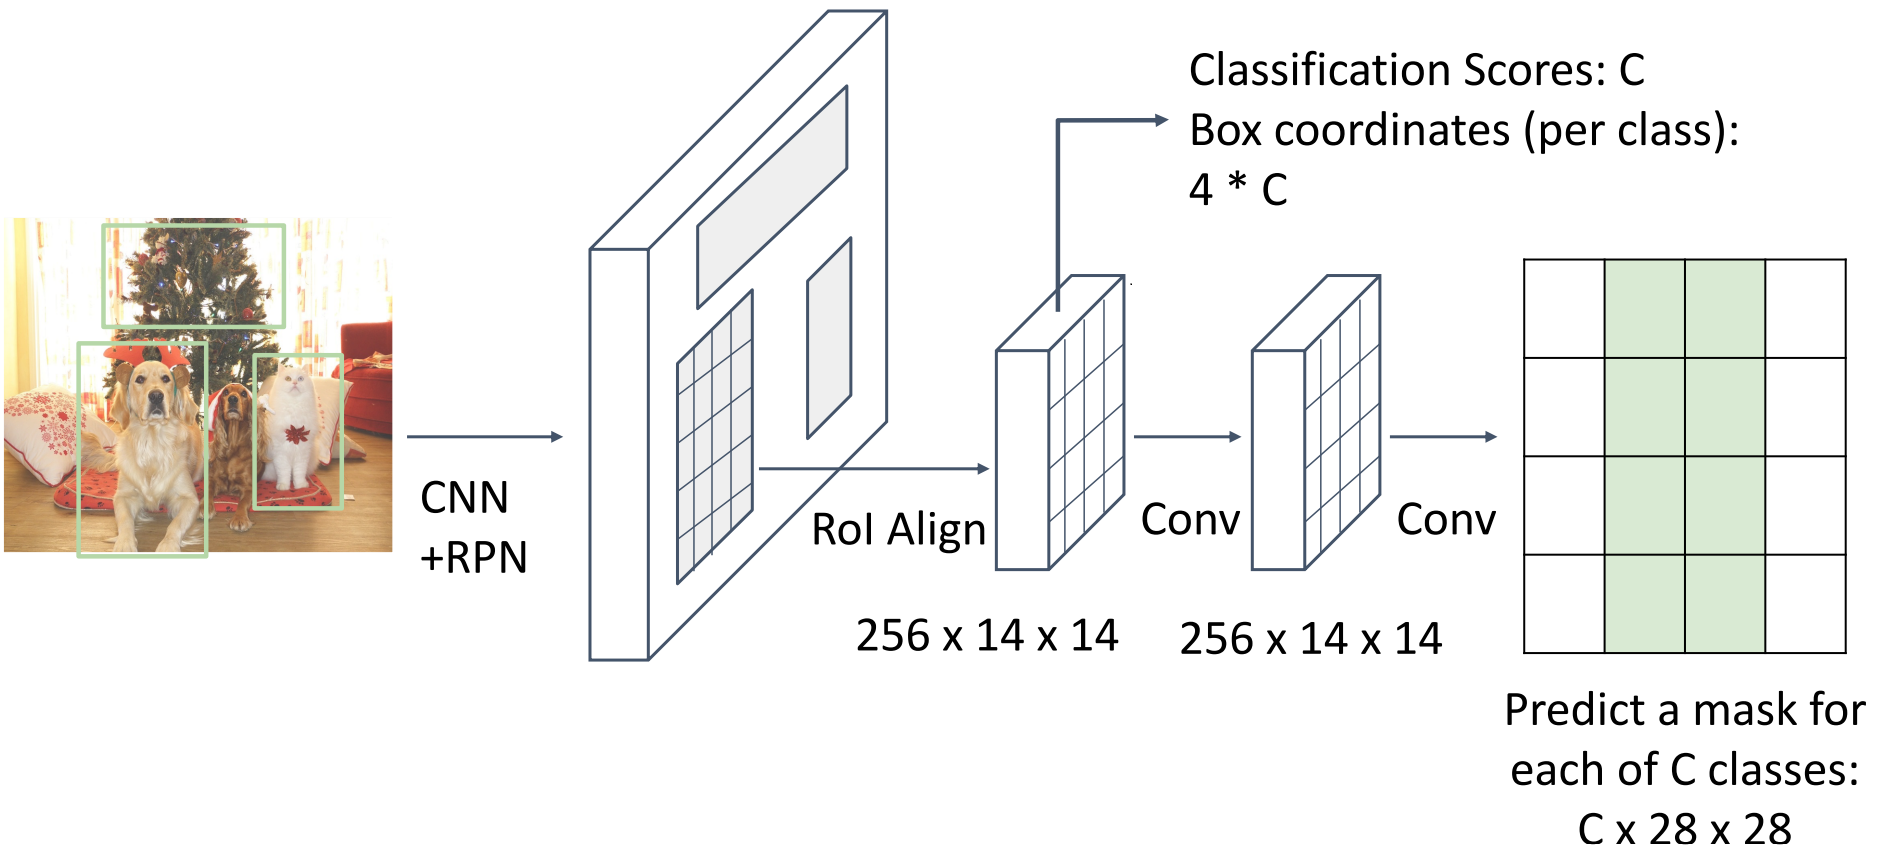
\includegraphics[width=1.0\textwidth,height=1.0\textheight,keepaspectratio]{images/object-detect/ins_7.png}
        \end{figure}
    }

\framebreak

    \textbf{Advantages of Mask R-CNN}
    \begin{itemize}
        \item \textbf{Simplicity}: Simple to train
        \item \textbf{Performance}: Outperforms previous methods, works almost in real-time
        \item \textbf{Efficiency}: Very efficient, small overhead compared to Faster R-CNN
        \item \textbf{Flexibility}: Can perform detection and estimation tasks simultaneously
    \end{itemize}
\end{frame}

\begin{frame}{Mask R-CNN: Example Training Targets}
    \only<2>{
        \begin{figure}
            \centering
            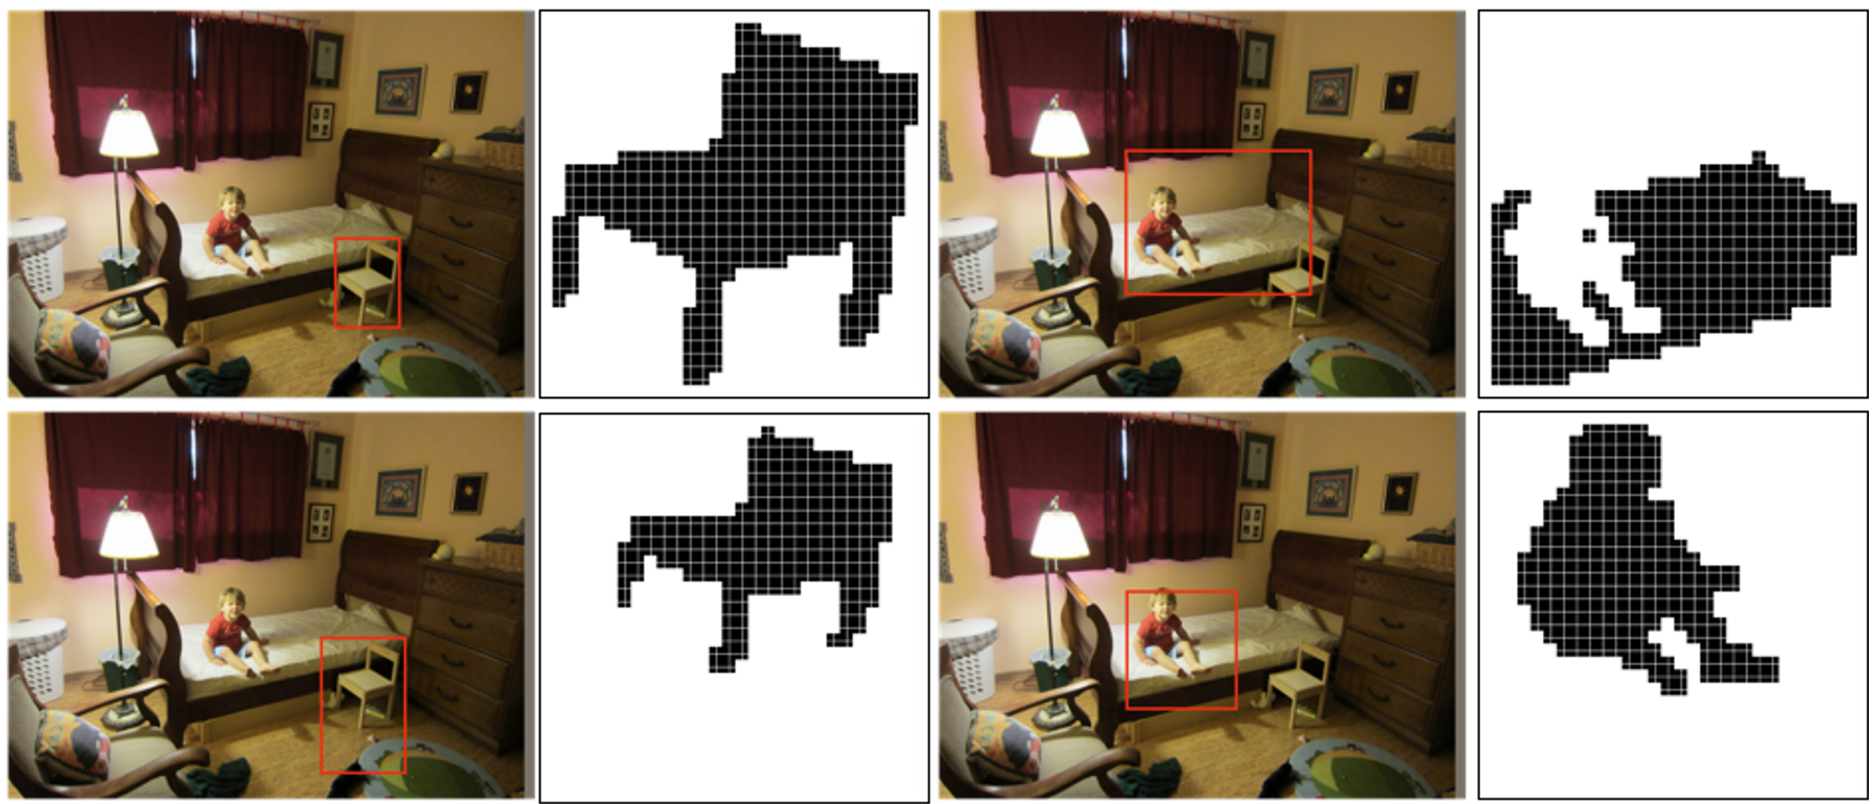
\includegraphics[width=1.0\textwidth,height=1.0\textheight,keepaspectratio]{images/object-detect/ins_8.png}
        \end{figure}
    }
\end{frame}

\begin{frame}{Mask R-CNN: Very Good Results!}
    \begin{figure}
        \centering
        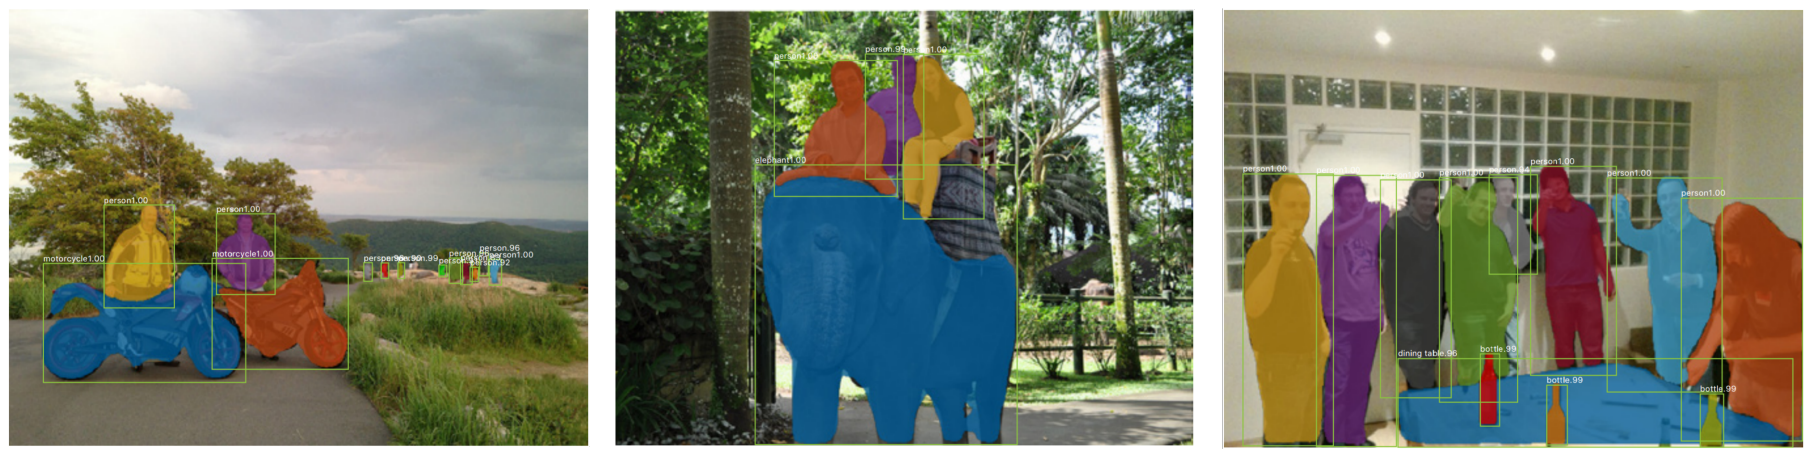
\includegraphics[width=1.0\textwidth,height=1.0\textheight,keepaspectratio]{images/object-detect/ins_9.png}
    \end{figure}
\end{frame}